\documentclass[10pt,twocolumn,letterpaper]{article}
%% Welcome to Overleaf!
%% If this is your first time using LaTeX, it might be worth going through this brief presentation:
%% https://www.overleaf.com/latex/learn/free-online-introduction-to-latex-part-1

%% Researchers have been using LaTeX for decades to typeset their papers, producing beautiful, crisp documents in the process. By learning LaTeX, you are effectively following in their footsteps, and learning a highly valuable skill!

%% The \usepackage commands below can be thought of as analogous to importing libraries into Python, for instance. We've pre-formatted this for you, so you can skip right ahead to the title below.

%% Language and font encodings
\usepackage[english]{babel}
\usepackage[utf8x]{inputenc}
\usepackage[T1]{fontenc}

%% Sets page size and margins
\usepackage[a4paper,top=3cm,bottom=2cm,left=3cm,right=3cm,marginparwidth=1.75cm]{geometry}

%% Useful packages
\usepackage{amsmath}
\usepackage{graphicx}
\usepackage[colorinlistoftodos]{todonotes}
\usepackage[colorlinks=true, allcolors=blue]{hyperref}
\usepackage{natbib}
\bibliographystyle{unsrt}
%% Title
\title{
		\usefont{OT1}{bch}{b}{n}
		\normalfont \normalsize \textsc{STEM Fellowship Big Data Challenge 2020} \\ [10pt]
		\huge The Effect of the Spread of Anti Vaccine Ideology on the Internet in the Rise of COVID-19 Cases \\
}
\selectlanguage{english}
\usepackage{authblk}
\author[1]{Aditi Das}
\author[1]{Tanya Ghai}
\author[1]{Mit Patel}
\author[2]{Rudra Patel}
\affil[1]{McMaster University, Hamilton, ON, Canada}


\begin{document}
\maketitle

\begin{abstract}

Coronavirus disease or COVID-19 has been a catalyst to redefine the way of life around the world. It was classified as a world-wide Public Health Emergency by the World Health Organization (WHO) on 30 January 2020 (CPHA, 2021a). Ever since, there have been many governments as well as pharmaceutical companies that have tried to find a vaccine to help tackle the exponentially increasing number of cases of COVID-19 around the world. Among those there are the mRNA vaccines like Pfizer, Moderna and viral vector vaccines (Centers for Disease Control, 2021) . There has been extensive research put into determining the effectiveness of these vaccines. However, vaccines have been a controversial topic on the internet and more precisely in various social media platforms. There is a growing community of those who classified themselves as anti-vaxxer who are hesitant about taking the vaccines for various reasons including their skepticism about the effectiveness, fear of fatal side effects or firm belief in many conspiracy theories. This paper analyzes the use of hashtags and search terms on social media that contributes to the spread of COVID-19 misinformation and uses Python and Excel as well as external sources to gather graphical representations of the data. These trends are then studied to determine the effects of the rate of spread of false information on the rise of COVID-19 cases. It was found that on twitter there is a higher rate of occurrence of hashtag #covidvaccine, however any sort of anti-vaccine hashtags are blocked by the social media platform, which prevents the spread of misinformation to an extent. Sentiment analysis of about 207006 tweets showed that while the majority of users had a positive attitude towards the COVID vaccine, there were a significant number of people who were skeptical about the vaccine. Finally, analysing google trends show a surge in the use of search terms related to anti-vaccine ideology in December 2020, right after the COVID vaccines were first approved by FDA. This again confirms the presence of public mistrust towards the vaccine. 
    
There are some limitations to our study, enough data such as the location of false tweets needs to be collected to prove the correlation between the spread of misinformation of anti-vaccine ideology and the rise of covid cases in certain locations, finding the number of bot accounts on Twitter which is contributing to spread of misinformation, and access to online resources, databases, surveys, and questionnaire.  The study performed in this paper would be an informative source of information for related studies in future and implement ways to reduce the spread of misinformation.


\end{abstract} \\ 
\\ 
\vspace{\baselineskip}
{\textbf{Keywords} \\
Common search terms, common hashtags, anti-vaccine, sentiment analysis, trend }

\section{Introduction}

The news of Coronavirus engulfed the world from December 31, 2019 and was declared to be a Public Health Emergency of International Concern by WHO on 30 January 2020 (CPHA, 2021a). COVID-19, as it is commonly called, causes Severe Acute Respiratory Syndrome (SARS) (CPHA, 2021a), which gives rise to symptoms like coughing, shortness of breath, or body temperatures above 38 degrees celsius (CPHA, 2021b). The most commonly used method of testing for COVID-19 is through nasal mid-turbinate or NMT swab. If tested positive, one has to self isolate for 14 days and those who have come into close contact must do the same (CPHA, 2021b). Due to the rapidly increasing cases worldwide, it was declared as a global pandemic on 11 March 2020 (CPHA, 2021a). Currently, 168,866,145 people have been infected with COVID-19 as of May 26, 2021 with 3,506,304 deaths and 150,476,302 recovered (Worldometer, n.d). Given this information, it is evident that this phenomenon has affected and implicated mental and physical damages to those affected. It has changed the way of life for everyone around the world, and has also redefined societal norms, with schools and work being done remotely, as well as the need to wear masks. In such a critical time when the world was in dire need of strong leadership, the response from the Government and other influential organizations have been a controversial topic, which caused many to have developed personal biases regarding the response of health organizations (Loomba, Figueiredo et al, 2021). 

The greatest response in combating COVID-19 has been through vaccination programs. When COVID-19 was deemed a pandemic, many global health and pharmaceutical companies as well as government organizations took charge to develop a vaccine that can help individuals build a strong immune response to infection by the virus. mRNA vaccines are some of the first COVID-19 vaccines that were authorized for use in the United States (Centers for Disease Control and Prevention, n.d).  Unlike many other previous vaccines that injected a weakened virus into the body to generate an immune response, mRNA vaccines are focussed on teaching cells how to create a “spike protein” that will trigger an immune response (Centers for Disease Control and Prevention, n.d). When the immune system detects an unwanted protein is present, it commences a response by creating antibodies training our bodies to counter the infection similar to COVID-19. Additionally, the benefit of such a method is that the antibodies would remain in the body afterwards for future infections. The most prominent vaccines that are in distribution in North America are the mRNA vaccines - Pfizer and Moderna. These types of vaccines require 2 doses,  which are given roughly 3 to 4 weeks apart (Centers for Disease Control and Prevention, 2021). Other common COVID-19 vaccines include AstraZeneca and Johnson & Johnson, however, due to the increase in health concerns of people who have taken those vaccines, they are not being administered in Canada. There has always been controversy for the effectiveness and safety of vaccines for COVID-19 as people have been uncertain about the side effects it can cause to those who choose to take it due to the little perceived time for testing. There is a huge group of people who are hesitant about taking the COVID-19 vaccine, either because they are concerned about the purity of the ingredients of the vaccine or the potential side effects (Loomba, Figueiredo et al, 2021). One study mentions that social acceptance of a potential vaccine among peers and social network members is a contributing factor in one’s opinion of vaccines (Loomba, Figueiredo et al, 2021). There is also a general distrust towards corporations associated with vaccine production since these companies are typically known to prioritize profits by downplaying side effects or exaggerating benefits to maximize their sales (Loomba, Figueiredo et al, 2021). The lack of trust in government policymakers is also another factor contributing to hesitancy towards vaccination (Loomba, Figueiredo et al, 2021). 

Due to the Internet and social media, the connectivity has become much faster. The world has become global. The world has become a global village where knowledge, ideas, information and everything flows quite easily from one place to another. The Internet or social media has become quite useful in our daily public life as well. Social Media is a great power today. It is the driving force behind the power of public opinion today. Social Media has given the power and voice to the grass root level of society. It is the voice of common people against injustice, COVID-19 related initiatives (anti-mask campaign) and for public rights (Johns Hopkins). Thus, these days information can spread to millions of people in a fraction of seconds, whether the information is right or wrong. 

Specifically, a lot of misinformation about covid-19 vaccine has spread. Some of which will be outlined below. First myth is that, people believed that researchers rushed  the development of the COVID-19 vaccine, so its effectiveness and safety cannot be trusted. However, the fact is  vaccine studies proved that it is 95 percent effective- and reported no serious or life-threatening side effects (Johns Hopkins). Second myth is that getting the COVID-19 vaccine means people can stop wearing their mask and the CDC revised safety guidelines for those who are fully vaccinated against the coronavirus and state that fully vaccinated people can resume activities without wearing a mask or physically distancing, except where required by federal, state, local, tribal, or territorial laws (Johns Hopkins). Third myth is that the side effects of the COVID-19 vaccine are dangerous. However, the fact is the CDC confirms that The Pfizer and Moderna COVID-19 vaccines can have side effects, but the vast majority are very short term —not serious or dangerous. Some minor symptoms which are seen after getting a vaccine means that it is working to stimulate your immune system (Johns Hopkins). 

In the current society, social media acts as a catalyst for the spread of (mis)information about any topic as those who have more influence on social media spread unproven information about topics they are not experts in (Igoe, 2019). It is a place where people can freely express their opinions and due to lack of filtering of information, social media can play a role in fueling vaccine hesitancy by spreading misinformation and thus, polarizing public opinion. Even since the pandemic started there has been a spread of false news, such as people dying from the side effects of COVID-19 vaccines, the virus being a government conspiracy or a bioweapon. While many people see vaccines with a positive point of view, there are those known as “anti-vaxxer” that create a challenge for health officials to point out the truths and to debunk any misinformation. Often as a result of social media and the influence and addition of opinions, information is misinterpreted causing mass panic and a difficult time for Public health to communicate the facts to the general public. Studies have shown that misinformation obtained through social media lowers the willingness in people to take the vaccine (Latkin, Dayton et al, 2021). Vaccination campaigns are less likely to work on people who already have been exposed to misinformation (Latkin, Dayton et al, 2021). It is difficult to undo the preconceived ideas once they have been embedded into a public’s consciousness (Latkin, Dayton et al, 2021). 

This paper endeavours to investigate the effect of spread of anti-vaccine ideology on the rise of COVID cases through analysis of data obtained from twitter and google trends and analysis of the data through coding softwares. It was hypothesized that social media platforms like twitter and google searches have a high occurrence of search terms or hashtags that are related to anti-vaccine ideology and have a big role in influencing public attitude towards vaccines. 

\section{Materials \& Methods}

There are many ways to handle data. This paper strives to determine the correlation of the misinformation spread about the vaccines, decreasing in the amount of doses administered to the public, and the amount of COVID-19 cases rising. In order to gather the information regarding the common vaccine hashtags, a vaccine database provided by Kaggle was utilized. Thereafter, to create Table 1, Google Collab was used to analyze the .csv files that were retrieved from Kaggle. The .csv file was opened using the Panda library and the hashtag column was read and the number of occurrences of certain chosen hashtags related to the anti-vaccine movement was determined with that data. 

The pie chart (Figure 5) was also created using the same database used to find the kind of accounts that uploaded the posts about vaccines. Using the Excel data analysis feature, it was determined the numbers of accounts that were unverified and verified.

Google trends is a powerful tool to determine the interest of certain searches over time. Using this tool, most common searches were analyzed. Most of these searches were related to anti-vaccine or negative connotation regarding the COVID vaccine and using the interest graphs, it was comparable to doses administered as well as to get a general understanding of the thoughts that many people had regarding the vaccines.

Many of the graphs used were retrieved from Google and other credible sites in order to get information about the number of cases of COVID-19 that were tested positive over a period of time in Canada (Figure 2) and United States (Figure 1). To see a correlation between the cases of COVID-19 and the number of vaccines administered, Figure 4 and 5 were found which show the number of vaccines that each country in Canada and US respectively administered over a period of time.

\section{Results}

\textbf{3.1 Number of COVID-19 Cases in US and Canada}

As seen in Figure 1, there is a spike of cases of COVID-19 in the United States between November 2020 to January 2021, peaking at 300 thousand cases per day. This was also the time when the Pfizer-BioNTech COVID-19 Vaccine and Moderna COVID vaccine were discovered and eventually approved by the FDA. The surge in the number of cases shows a slow decline from February 2021. Canada shows a similar trend as the US between November 2020 and January 2021, as shown in Figure 2, peaking at around 11 thousand. While the daily cases drop slightly during February, there is a drastic increase in the rate of daily occurrences from March till date. 


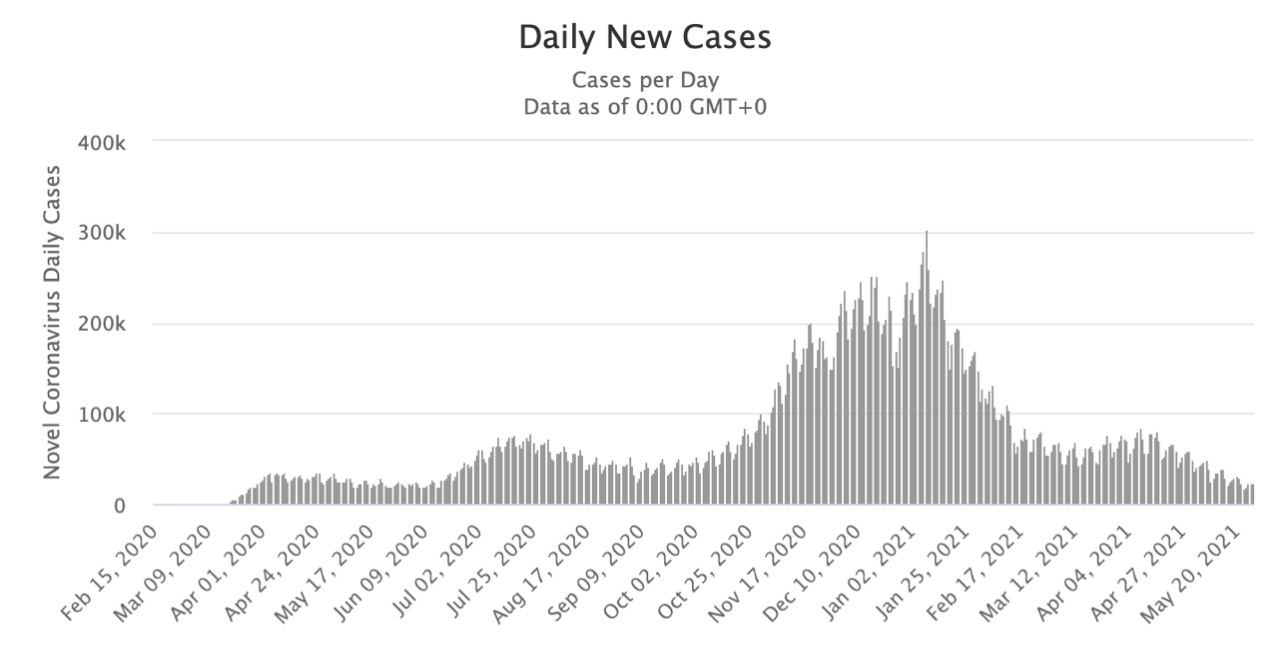
\includegraphics[scale=0.30]{fig1.png}
\caption{Figure 1: A timeline of Number of COVID-19 cases in United States of America from February 2020 to May 2021}

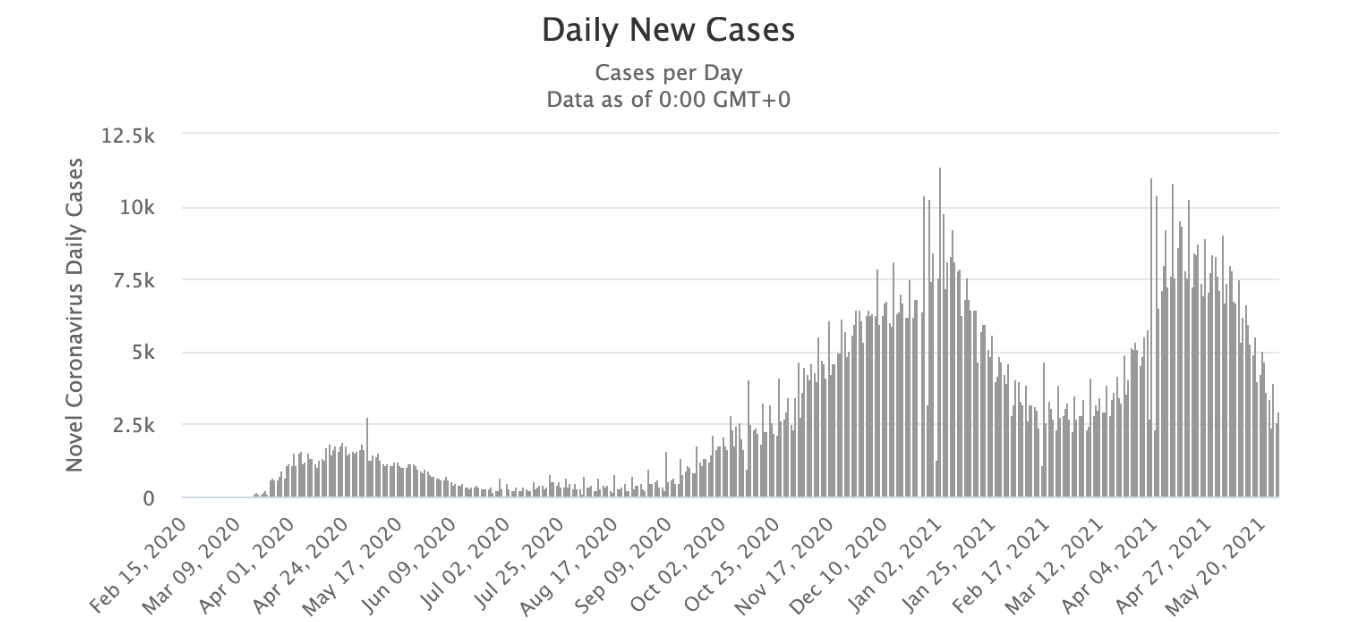
\includegraphics[scale=0.30]{fig2.png}
\caption{Figure 2: A timeline of number of COVID-19 cases in Canada from February 2020 to May 2021}

\textbf{3.2 Number of People Receiving the COVID-19 Dose of Vaccination}

Figure 3 shows a rising trend in the number of doses administered in Canada from January 2021 to May 2021.The rate of vaccine administration was a slow process in the beginning. From January to March, only about 4 million dosages were administered. However, this rate started drastically increasing towards the end of March and by the end of May a little above 22 million people were vaccinated. In the USA, a greater number of doses were administered per day in comparison to Canada and the rate of vaccination was faster as well. By mid-January, the US was able to vaccinate about 1 million people per day on average. Overtime, a rapid increase in the trend can be noticed, which peaked to 4.5 million doses per day around mid-April. From that point, the rate of dosage administration shows a declining trend.


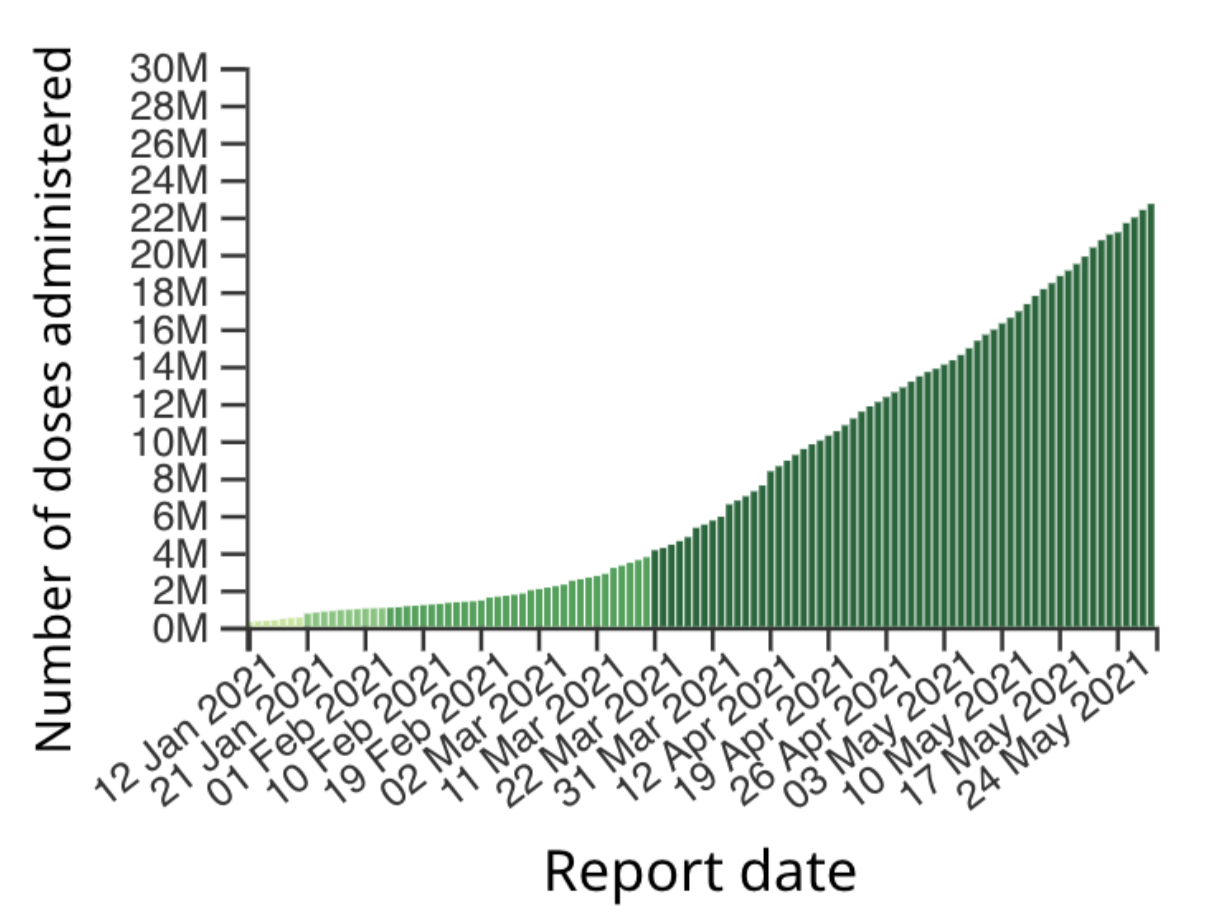
\includegraphics[scale=0.33]{fig3.png}
\caption{Figure 3: Cumulative number of COVID-19 vaccine doses administered from January 2021 to May 2021 in Canada.}

\vspace{\baselineskip}

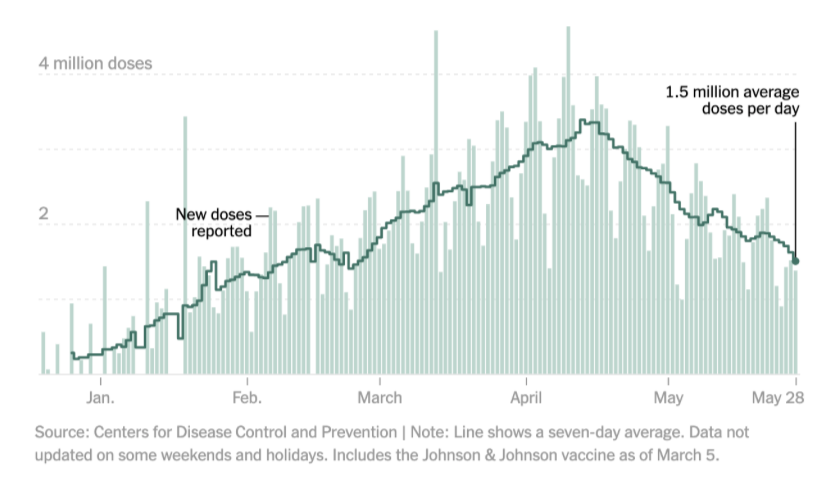
\includegraphics[scale=0.5]{fig4.png}
\caption{Figure 4: Number of COVID-19 Vaccines administered in the United States of America from January 2021- May 2021}

\vspace{\baselineskip}

\textbf{3.3 Number of Accounts Verified versus Unverified on Twitter}
\vspace{\baselineskip}

To analyse the number of verified accounts on twitter in comparison to that of the unverified account, a total of 206,993 accounts were analysed. It was found that 187533 accounts, which is 91 percent of the total data, were unverified whereas 19460 accounts or 9 percent were not verified, as shown in Figure 1. While this data is not directly related to COVID-19 vaccine misinformation, it is hypothesized that a portion of the unverified accounts are controlled by bots that can potentially be programmed to spread false information. Due to limitations in regards to accessible data, it was not possible to confirm the exact number of bot profiles. 

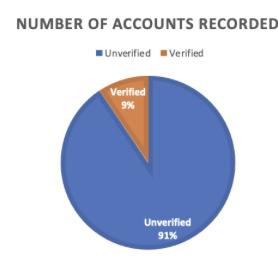
\includegraphics[scale=1.45]{fig5.png}
\caption{Figure 5: Number of Accounts Verified versus Unverified on Twitter}

\vspace{\baselineskip}
\textbf{3.4 Usage of Common Hashtags Related to Anti-vaccine Ideology}

\vspace{\baselineskip}

A total of 200 COVID-19 related hashtags were analysed, out of which the most-used  and relevant ones are reported in this paper. Prior to analysis, a moderate to large amount of occurrence for anti-vaccine hashtags was expected. While there are a significant amount of searches for COVID vaccine related information, the limited number of occurrences of anti-vaccine and vaccine misinformation linked hashtags was an unexpected discovery. Upon further investigation, it was found that social media platforms like twitter, Instagram etc. block the use of search terms that are associated with misinformation spread, limiting the rate of spread to an extent. 

\caption{Table 1: Usage of common Hashtags by individuals on Twitter}
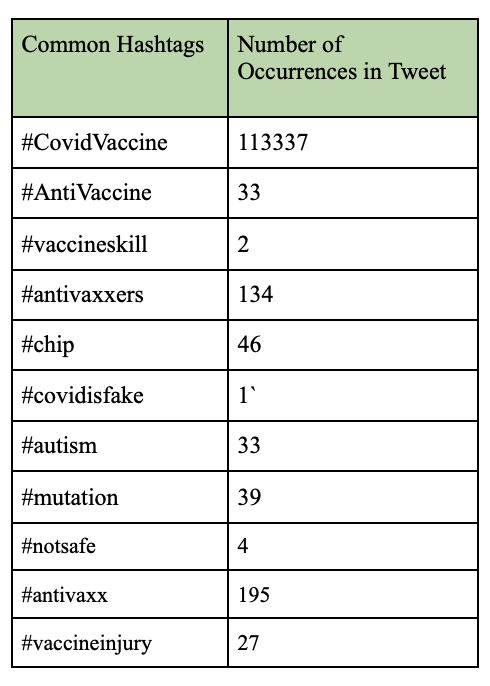
\includegraphics[scale=0.8]{Table 1.png}

\textbf{3.5 Sentiment Analysis In Relation To COVID-19 Vaccine on Twitter 207006}

The COVID vaccine discovery evoked a wide range of emotions among the general population. A sentiment analysis conducted on Twitter provides information about people’s sentiment towards vaccines. The sentiment score is dependent on the Python library that was used to analyse the tweets for sentiments by Pulkit Saxena from Kaggle.  A total of 207006 tweets were analysed and  it was found that a significant number of users had a positive reaction as well as reaction of joy, anticipation, trust and surprise towards the COVID-19 vaccines. However, there were many tweets that displayed negative reactions including feelings of anger, fear, disgust and sadness. A big number of negative tweets is very likely to contribute to the spread of more false information and hesitancy towards the vaccine. 

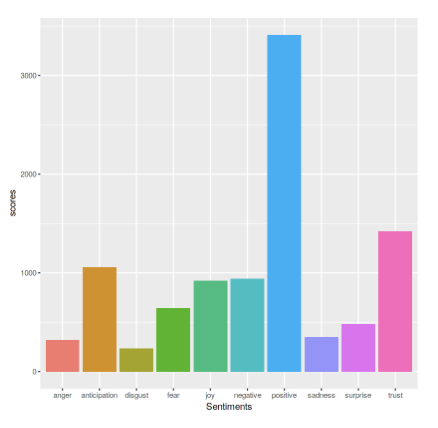
\includegraphics[scale=1.3]{fig 6.png}
\caption{Figure 6: Sentiment Scores from  Individuals about the COVID-19 Vaccine on Twitter}

\vspace{\baselineskip}

\textbf{3.6 Timeline of Use of Common Search Terms Related to Anti-Vaccine Ideology on Twitter}

\vspace{\baselineskip}

A total of 100 common search terms used worldwide that are related to COVID-19 anti-vaccine ideology were analysed, out of which, 5 most frequently used terms are reported on the Figures 7.a and 7.b. The others were excluded from the list due to the extremely low rate of occurrence. A common observable trend between these 5 search terms is that the frequency of occurrence has increased since December 2020, which is also when the COVID-19 vaccines were approved. Figure 7.a shows that people are most likely to search for the side effects of COVID-19 vaccine instead of the rate of mortality caused by it. Figure 7.b confirms that a significant number of people were concerned with the safety of the vaccines, which is inferred from the frequent use of the search term “is COVID vaccine safe?”. A large group of individuals were also against the administration of the COVID vaccine and were actively seeking information about “anti-vaccine” ideology. The spread of misinformation is also evident from the rate of occurrence of the search term “covid chip”, implying the fact that a significant number of individuals were concerned with a microchip being injected into their bodies through the vaccines. 

\vspace{\baselineskip}
\vspace{\baselineskip}
\vspace{\baselineskip}

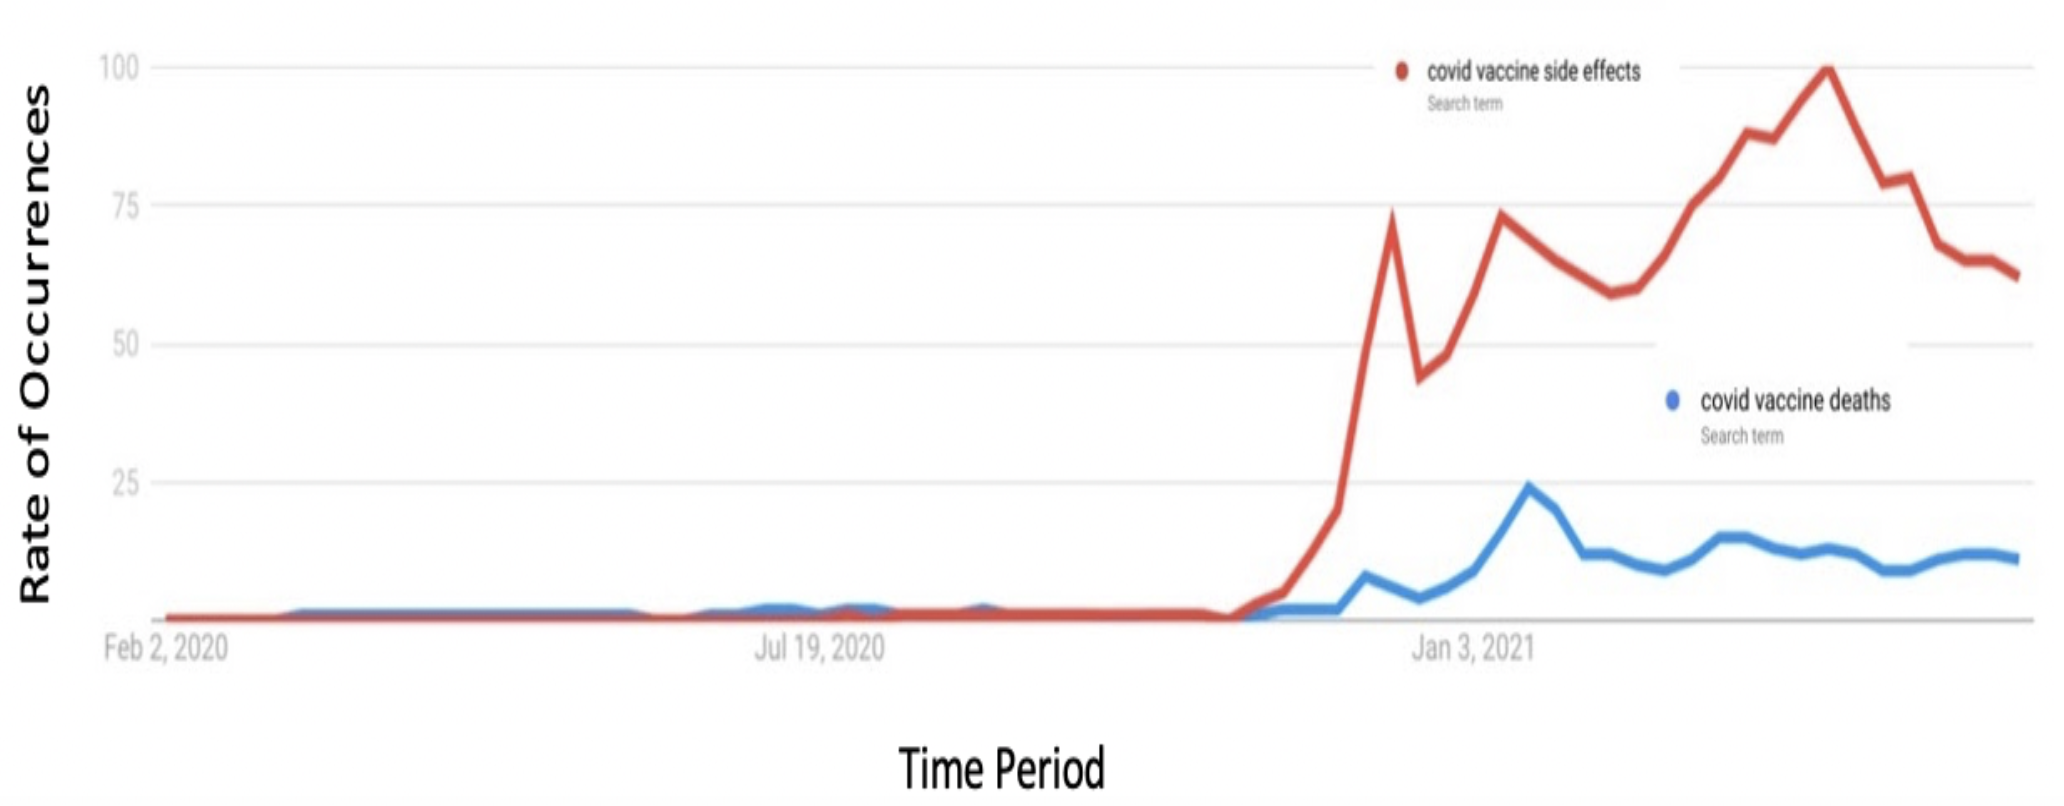
\includegraphics[scale=0.2]{fig7a.png}
\caption{Figure 7.a: Rate of occurrences of search terms “covid-vaccine side effects” (red) and “covid vaccine deaths” (blue) at different time periods from February 2020 to May 2021. }

\vspace{\baselineskip}

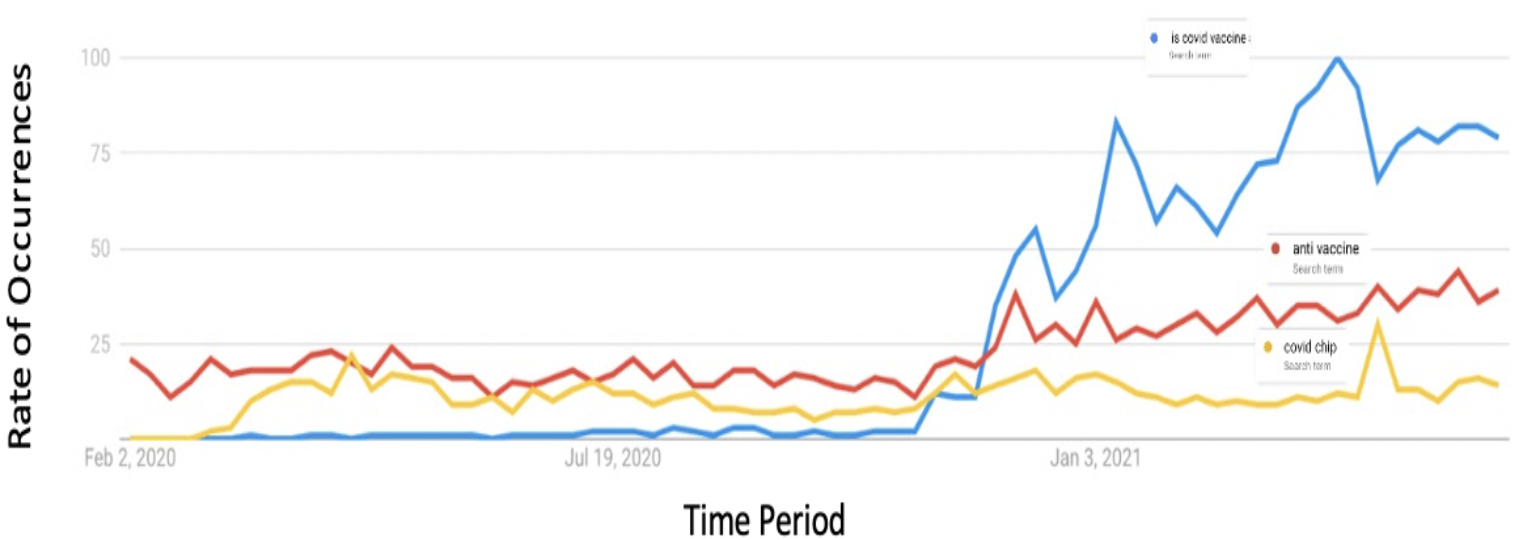
\includegraphics[scale=0.24]{fig7b.png}
\caption{Figure 7.b: Rate of occurrences of search terms “is covid vaccine safe” (blue), “anti vaccine” (red)  and “covid chip” (yellow) at different time periods from February 2020 to May 2021}

\section{Discussion}
The overall purpose of this study was to examine the anti-vaccine ideology that has spread its influence across various social media platforms leading to public health misinformation. Statistical data has been collected across a variety of sources such as google trends, twitter etc. that examine the correlation between COVID-19 incidence rates post development and FDA approval of the administration of the mRNA COVID-19 vaccine. Upon the examination of the obtained results, it can be concluded that a relatively large proportion of the population was resentful and fearful of being administered the COVID-19 vaccine. This fear and choice to not receive the vaccine stems from a multitude of factors. This includes a lack of trust in the efficacy and ingredients, the fear of adverse symptoms, and the idea of "politicized medicine" (Chou, Gaysynsky et al, 2020 ). This fear arises from public health information which stems from social media.
 
 
Over the past century, the development of social media platforms have revolutionized the vast array of locations in which individuals access online information. The controversy behind the accuracy of information on social media has been a hot topic due to the relevance of bias that is brought in from online information from these sources. Research suggests that social media has led to a spike in the accessibility of public health misinformation, such as its amplification in the false information on vaccines. Public health misinformation is defined as a health related claim or fact that is false based on current scientific research (Chou, Gaysynsky et al, 2020).. Health misinformation on social media, therefore, urgently requires greater action from those working in public health research and practice. 
Upon the examination of figure 1 and figure 2 which depict the number of COVID-19 cases across the time frame of February 2020 and may 2021 for the United States and Canada respectively, it can be the seen that there is a spike In the number of COVID-19 cases in the months of December 2020 and January 2021. This was also the time when the Pfizer-BioNTech COVID-19 Vaccine and Moderna COVID-19 vaccine were discovered and eventually approved by the FDA. The major reason why both countries experienced a spike in the number of COVID-19 cases during this 2 month window (December-January) could be because of the Christmas Holidays / Winter Break and the New Years (Guglielmi, 2020). During this period of time a greater number of individuals come into social contact with each other through public events and social gathering interactions with family and friends. It is hypothesized that this spike in the number of COVID-19 cases during this time span is due to a large portion of the population failing to maintain social distance. However, during the months of March 2021, April 2021 and May 2021 Canada had experienced a second significant raise in COVID-19 cases while the U.S did not experience this change. The major reason why Canada experienced its third wave of COVID-19 is because of the development of the novel variant B.1.1.7 which first originated in the United Kingdom (Lowrie, 2021). It is shown that 5154 of the new cases in the month of March were transmissible variants (Lowrie, 2021). It is also possible that Canada. experienced this spike in COVID-19 due to the seasonal change from the winter to the spring/summer months. This seasonal change drives more individuals to go outside and attend more social gatherings and thus break the governed rules and social distancing restrictions.
Figure 3 and 4 examines the number of people that receive the COVID-19 vaccination dose between January 2021 and May 2021. It can be seen that in the first few initial months there were many doubts and hesitancy regarding vaccines in the earlier stages of vaccine circulation, but overtime the confidence in the vaccine and the availability may have increased, resulting in the increase in the number of doses. In the U.S after April however the number of doses began to decline due to the possibility of public health misinformation.
According to Figure 5, 91 percent of the accounts on twitter are unverified and only 9 percent of the accounts are verified. 91 percent accounts for around 187533 accounts on twitter. However, this data does not relate to how covid-vaccine misinformation is spread, but it is known that a large portion of the unverified accounts are controlled by bots. One study suggested that around 9-15 percent active Twitter accounts were bots. In 2019, they found around 6 billion fake accounts.  (cite).  On social media, there are automated accounts that are run by bots and are programmed to send out specific types of information through many ways (Wiggers, 2020). Some ways include, trying to get something to trend, artificial amplification of conversations, including through creating multiple or overlapping accounts, generating, soliciting, or purchasing fake engagements, engaging in bulk or aggressive tweeting, engaging and following, bots can use hashtags in a spammy way (Wiggers, 2020). Thus, this way  bots can play a key role in the spread of fake news about covid-19 vaccine. The studies identified dozens of bots on Twitter , particularly within communities where “low-credibility” sources and “suspicious” videos proliferate (Wiggers, 2020). Thus, there is evidence that bots do play a role in the spread of misinformation on social media. 

Table 1 depicts  covid 19 related, most relevant hashtags out of 200 which were analyzed. Due to so many myths as discussed earlier in this paper, a large amount of occurrences for anti-vaccine hashtags was expected. It was found that there was a significant amount of searches about covid vaccine topics, but there were limited occurrences of anti-vaccine and vaccine misinformation linked hashtags on twitter. After investigating more, it was found that a lot of social media platforms lock the use of such hashtags and terms associated with spreading of misinformations. By looking at the table, it is still evident that around 113, 855 total tweets were there for anti-vaccine related hashtags. This number is not huge, but it also shows many people are interacting with such tweets and there is still somewhat misinformation spread through such posts in the media. 

Figure 6 depicts a sentiment scores analysis on how people feel about  the COVID-19 vaccine on Twitter. When the COVID-19. vaccine came out in December, a wide range of emotions among the general population was observed through twitter. Lot of people did have a positive reaction towards the COVID-19 vaccine. However, many felt emotions such as anger, disgust, fear, negative reaction, sadness. There was a low amount of trust in COVID-19 vaccine as well. Thus, this shows that there has been a spread of misinformation regarding COVID-19 vaccine when the vaccine was first developed as many did not trust and had a negative reaction (figure 6). 

Figure 7.a showcases a timeline of common search terms related to anti-vaccine ideology on twitter. Google trend analysis showed  a total of 100 common search terms being used worldwide that are related to covid-19 anti-vaccine ideology, out of which, only 5 were most popular terms as reported on the Figures 7.a and 7.b.  The others were excluded from the list due to the extremely low rate of occurrence. Figure 7a, shows the rate of occurrences of only two search terms “covid-vaccine side effects” (red) and “covid vaccine deaths” (blue) at different time periods from February 2020 to May 2021. One common trend is seen that the frequency of these both terms increased (a spike in graph) around December 2020, which is also when the COVID-19 vaccine were approved. Thus, it is evident that spread of misinformation has led to delay in the population not being able to accept the vaccine and trust the government as the previous graphs show that still a lot of people didn't get covid vaccine doses around early stages of when covid vaccine came out. Moreover, as the graph shows, a large group of individuals were also against the administration of the covid vaccine as they were actively seeking information about “anti-vaccine” ideology. 

In figure 7.b, it is seen that the majority of people have searched on google based on the google trends results "is covid vaccine safe". This high volume of searches indicate that many individuals in the population lack trust for the efficacy of the COVID-19 vaccine and are highly fearful despite the information given out by individuals and parties with a high level of credentials such as the government. "anti vaccine" is also another highly searched topic on the internet as people are looking for valid reasons to not get vaccinated. 

In the presence of a future global pandemic, a variety of methods can be used to reduce the spread of public health misinformation which causes a lapse in judgment within the general public on what is the correct health measure that needs to be taken. A few methods include improving ehealth literacy, use the internet and google search engine as a collaborative tool with physicians, strengthening the signal of source quality found online, and promoting public figures to spread increasingly accurate information on sustainable health measures. (Swire-Thompson & Lazer, n.d.). 

There are some limitations to our study, one of them includes that it remains unclear to the extent to which our explanations are concrete.  Enough data needs to be collected to prove the correlation between the spread of misinformation of anti-vaccine ideology and the rise of covid cases. For some of our data, enough information was not available as to which location the false tweets were spreading from  to prove that the certain location has a rise of covid 19 cases due to the false tweets from that certain location. 

Secondly, we couldn't confirm which accounts from all the unverified accounts (91 percent) were bots. Sometimes, bots can be programmed to increase the spread of misinformation.  Enough resources were not available to implement an AI for the detection of the number of  bot accounts on Twitter. Thus, the data and the results might be skewed as the spread of misinformation could be higher than seen in the results. 

Thirdly, access to online resources and databases were limited to making a firm conclusive statement. Data such as,  frequency of usage of anti-vaccine hashtags in certain locations where less number of individuals got vaccine (high cases), number of bots accounts on Twitter , and specific percentage of covid 19 cases influenced by anti vaccine ideology. In order to find the covid-19 cases benign influenced by anti-vaccine ideology, there should be availability of surveys and questionnaire responses by the public on this topic (reason for delay in getting vaccine or not getting vaccine)  or such surveys should be done to further improve the research conclusions.  


    Due to several limitations, this paper does not provide concrete evidence regarding the correlation between social media misinformation spread and rise of COVID-19 cases. However, findings of this study would be highly beneficial in performing social media analysis. Social media, undoubtedly, has a great role in impacting public opinion and spreading misinformation can lead to many public safety concerns. So it is crucial to conduct more research exploring the primary sources of misinformation in social media platforms, the group of people receiving these information and their attitude and subsequent response to it, the number of anti-vaccine hashtags used versus the change in COVID-19 cases in a specific time period and more. The research conducted in this paper would be an informative source of information for related studies in future. 


 


\section*{Conclusions}
    Coronavirus has made a huge impact in people's lives worldwide. Ever since January 2020,  all the governments around the globe as well as pharmaceutical companies  have tried to find a vaccine to help tackle the exponentially causes of covid-19 and death rates.  There has been extensive research put into determining the effectiveness of these vaccines. However, vaccines have been a controversial topic on the internet and more precisely in various social media platforms. On social media, there have been growing amounts of anti-vaxxers, people who don't have trust in the vaccine, fear of dangerous side effects, and  groups who believe in conspiracy theories and myths. After extensive research on various social media platforms, twitter was the platform where huge amount of misinformation regarding covid-19 vaccine was spreading which was leading to rise in covid-19 cases around January-March 2021. This is evident through our findings discussed above. Moreover, it was found that on twitter there is a higher rate of occurrence of hashtags related to anti-vaccine, however any sort of anti-vaccine hashtags are blocked by the social media platform, which prevents the spread of misinformation to an extent.  The key thing here is that in the initial stages of spread of misinformation, social media did not block such hashtags and must have contributed to rise in covid -19 cases. Once the hashtags were blocked, the spread of misinformation lowered, and more people started to get the vaccine.  Sentiment analysis of about 207006 tweets demonstrated  that while the majority of users had a positive reaction towards the COVID vaccine, however there were a significant number of people who were skeptical and had a negative response towards getting vaccine. Finally, analysing google trends proved that the anti-vaccine ideology  was getting very popular from December 2020; this contributed to an increase in spread of misinformation and leading to less people getting vaccine when the COVID vaccines were first approved by FDA around december. This also highlights the fact that there is a  presence of public mistrust towards the vaccine. If such a scenario arises in future, lessons should be learnt now so that public health misinformation spread can be reduced next time. Some ways to do that would be to block the use of hashtags and posts by the social media personnels, improving literacy, using google to work collaboratively with healthcare professional to put accurate information online, strengthening source of quality of the information presented online, and having public figures on social media promoting accurate information on health and safety measures. 
\section*{Acknowledgements}
The authors of this paper would like to acknowledge the STEM Fellowship for providing many resources and opportunities for the undergraduate students to help them in improving their research and data analysis skills. 

\bibliography{bibliography}
1. CPHACanadienne de Santé Publique. (2021, February 16). Review of Canada's Initial Response to the COVID-19 Pandemic.     https://www.cpha.ca/review-canadas-initial-response-covid-19-pandemic. 

2. CPHA. (2021, March 22). Government of Canada. Canada.ca. https://www.canada.ca/en/public-health/services/diseases/2019-novel-coronavirus-infection/symptoms.html

3. Centers for Disease Control and Prevention. (2021, May). Different COVID-19 Vaccines. Centers for Disease Control and Prevention.    https://www.cdc.gov/coronavirus/2019-ncov/vaccines/different-vaccines 

4. Centers for Disease Control and Prevention. (n.d.). Understanding mRNA COVID-19 Vaccines. Centers for Disease Control and Prevention. https://www.cdc.gov/coronavirus/2019-ncov/vaccines/different-vaccines/mrna.html.

5. Chou Sylvia, W.-Y., Gaysynsky, A., & Cappella, J. N. (2020, October). Where We Go From Here: Health Misinformation on Social Media. American journal of public health. https://www.ncbi.nlm.nih.gov/pmc/articles/PMC7532328/.  

6. Guglielmi, G. (2020, December 16). Coronavirus and public holidays: what the data say. Nature News. https://www.nature.com/articles/d41586-020-03545-1. 

7. Igoe, K. J. (2019, July 10). Establishing the Truth: Vaccines, Social Media, and the Spread of Misinformation. Executive and Continuing Professional Education. https://www.hsph.harvard.edu/ecpe/vaccines-social-media-spread-misinformation/.   

8. Johns Hopkins Medicine. (n.d.). COVID-19 Vaccines: Myth Versus Fact.https://www.hopkinsmedicine.org/health/conditions-and-diseases/coronavirus/covid-19-vaccines-myth-versus-fact. 

9. Latkin, C. A, Dayton, L, Yi, G., Konstantopoulos, A., & Boodram, B. (2021, February). Trust in a COVID-19 vaccine in the U.S.: A social-ecological perspective. Social science & medicine (1982). https://www.ncbi.nlm.nih.gov/pmc/articles/PMC7834519/. 

10. Loomba, S., Figueiredo, A. de, Piatek, S. J., Graaf, K. de, & Larson, H. J. (2021, February 5). Measuring the impact of COVID-19 vaccine misinformation on vaccination intent in the UK and USA. Nature News. https://www.nature.com/articles/s41562-021-01056-1. 

11. Lowrie, M. (2021, March 22). Cases of COVID-19 variants on the rise in Canada, fuelling concerns over the third wave. Coronavirus. https://www.ctvnews.ca/health/coronavirus/cases-of-covid-19-variants-on-the-rise-in-canada-fuelling-concerns-over-third-wave-1.5357592.     

12. Swire-Thompson, B., & Lazer, D. (n.d.). Public Health and Online Misinformation: Challenges and Recommendations. Annual Reviews. https://www.annualreviews.org/doi/full/10.1146/annurev-publhealth-040119-094127. 

13. Wiggers, K. (2020, December 21). Studies reveal verified social media users are fueling COVID-19 fake news. VentureBeat. https://venturebeat.com/2020/12/21/studies-show-bots-might-not-be-the-dominant-driver-of-covid-19-misinformation-on-social-media/. 

14. Worldometer. (n.d.). Coronavirus Cases.https://www.worldometers.info/coronavirus/.

\end{document}
